\chapter{Implementación y experimentos}
\label{ch:implementacion_experimentos}

\section{Obtención de datos}
\label{sec:obtencion-datos}

Para la obtención de datos se ha utilizado el \textit{DAO Analyzer dataset}~\cite{arroyo_dao_2024}, el único dataset sobre \glspl{dao} disponible en Kaggle o Zenodo a fecha de comienzo de este proyecto. Este dataset incluye datos de organizaciones en Aragon, DAOstack y DAOhaus, y en el que ha participado anteriormente el autor de este proyecto. Durante el desarrollo del TFM se ha modificado ligeramente el dataset para obtener la información textual (título y descripción) de las propuestas realizadas. Además, se ha aumentado este dataset con las \glspl{dao} de la plataforma Snapshot, utilizando parte de los scripts desarrollados durante la pasantía de verano de Andrew Schwartz en el Departamento de Ingeniería del Software e Inteligencia Artificial de la Universidad Complutense de Madrid, aunque también han necesitado ser modificados para descargar la información textual de las propuestas. Finalmente, los datos han sido publicados en Kaggle~\cite{tfm-dataset-text}.

Debido a que sólo se han explorado organizaciones de las plataformas Aragon, DAOstack, DAOhaus y Snapshot, en esta sección solo se explorará la obtención de datos de estas plataformas, aunque las herramientas utilizadas son capaces de más.

En la figura~\ref{fig:daos-census} puede verse un resumen de las fuentes de los datos y los procesos realizados para la elaboración del dataset.

\begin{figure}[tbh]
    \centering
    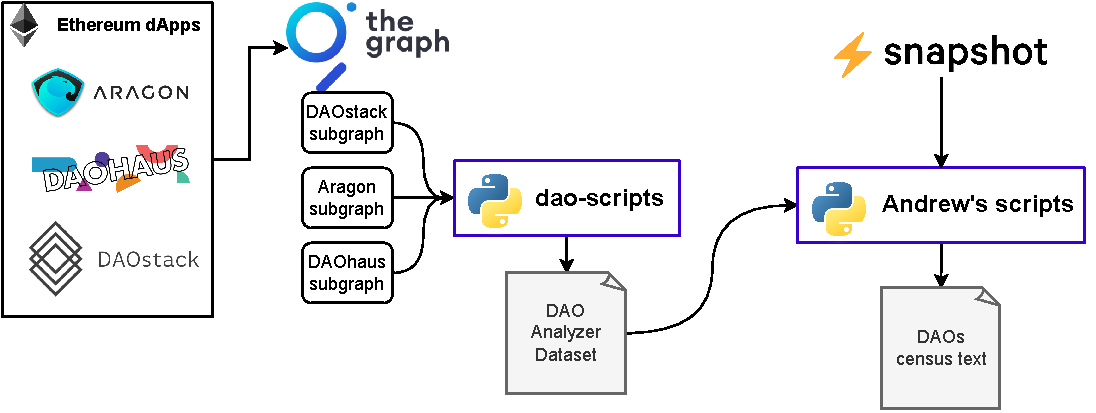
\includegraphics[width=\linewidth]{figures/04_implementacion/daos-census-Horizontal.drawio.pdf}
    \caption{Esquema de la obtención de datos de las plataformas para su posterior análisis.}
    \label{fig:daos-census}
\end{figure}

\subsection{Aragon, DAOhaus y DAOstack}

Para obtener los datos de las organizaciones de las plataformas Aragon, DAOstack y DAOhaus, el paquete dao-scripts~\cite{arroyo_dao-analyzer_2022} utiliza el servicio The Graph\footnote{\url{https://thegraph.com/}}, una plataforma que permite indexar y consultar datos de \glspl{dapp} de manera eficiente. Por como funciona la blockchain, la manera de conocer el estado actual de un programa en ejecución es descargarse toda la cadena de bloques y recorrerla bloque a bloque realizando las operaciones de reducción necesarias, de igual modo que para conocer el saldo de una cuenta bancaria es necesario computar todas las transferencias realizadas. The Graph provee de indexadores gratuitos que realizan esta tarea y dispone los resultados mediante una API en GraphQL, lo que evita tener un servidor indexando solo para nuestra aplicación. 

Para desplegar un subgrafo (cada uno de los repositorios de información indexada asociados a una \gls{dapp}) es necesario programar en Typescript el código que ejecutará el indexador, y para ello es necesario tener acceso al código fuente de los contratos inteligentes que forman la aplicación. Esta tarea ya la realizaron los creadores de las tres plataformas y por lo tanto los subgrafos ya están desplegados.

Sin embargo, muchas de estas plataformas han abandonado su desarrollo, por lo que ha sido necesario realizar cierto mantenimiento y en ocasiones añadir información necesaria para que pueda ser obtenida por los scripts en los subgrafos de Aragon y DAOstack.

El programa que obtiene los datos de The Graph, los empaqueta en formato Arrow o \gls{csv} y los sube a Zenodo y Kaggle se llama dao-scripts y el código en Python está disponible en GitHub\footnote{\url{https://github.com/Grasia/dao-scripts}}. Los datos son obtenidos diariamente con un GitHub action y actualizados tanto en Zenodo como en Kaggle, en un conjunto conocido como \textit{DAO Analyzer Dataset} y al que habría que añadir las organizaciones de Snapshot, como se explicará en la próxima sección. Los ficheros \gls{csv} que forman el conjunto de datos ocupan 130MB, de los cuales aproximadamente 100MB son la información textual de las propuestas.

\subsection{Snapshot}

En el caso de Snapshot, al ser una plataforma \textit{off-chain}, es decir, no desplegada en la blockchain, no podemos utilizar The Graph. Sin embargo, Snapshot utiliza su propia API GraphQL\footnote{\url{https://hub.snapshot.org/graphql}}, por lo que puede reutilizarse parte del código y de los algoritmos desarrollados en los dao-scripts. Sin embargo, debido al diferente esquema de la API~\cite{snapshot_snapshot_nodate}, además de problemas de escalabilidad inherentes a su popularidad y la gran actividad con la que cuenta, Andrew Schwartz hizo estos scripts casi de cero en Jupyter Notebooks. Posteriormente, realicé un \textit{fork} en GitHub\footnote{\url{https://github.com/daviddavo/daos-verano}} de dichos scripts, añadiendo algunas utilidades y, sobre todo, obteniendo la información textual de las organizaciones desplegadas en Snapshot.

Finalmente, estos notebooks combinan los datos del \textit{DAO Analyzer dataset} con los obtenidos de Snapshot para crear un nuevo conjunto de datos aumentado, denominado \citetitle{tfm-dataset-text} y disponible en Kaggle~\cite{tfm-dataset-text}. Este nuevo dataset está formado por ficheros en formato Parquet debido a su escala, y ocupa 3.63 GB. En este caso, el gran espacio ocupado es debido a la información sobre los votos, que ocupa aproximadamente 3.55 GB. La información textual de las propuestas ocupa tan solo 45 MB, y el resto de datos de las propuestas y organizaciones ocupa 32 MB.

La sección~\ref{sec:explora_datos} abordó la exploración de este conjunto de datos.

\section{Preparación de datos}

Para garantizar la reutilización del código de preparación de datos en todos los notebooks, se ha creado el módulo \url{src.datasets}, cuyo código está disponible en el GitHub del proyecto~\cite{davo_daviddavoupm-tfm-notebooks_2024}.

La extracción de los conjuntos de datos se realiza mediante la API de Kaggle, empleando el formato Apache Parquet para su almacenamiento. Dado el tamaño considerable de estos conjuntos, se ha optado por la utilización de DuckDB~\cite{raasveldt_duckdb_2023} para realizar consultas de filtrado, permitiendo así una manipulación eficiente de los datos. Posteriormente, se transforman los resultados en estructuras de datos manejables mediante Pandas DataFrame~\cite{mckinney_data_2010}.

Este proceso de preparación de datos se encapsula en el método \url{get} del módulo \url{src.datasets.daocensus}. Dicho método, al ser invocado con el nombre específico de la \gls{dao}, devuelve dos DataFrames distintos: uno que contiene todas las propuestas y otro que contiene los votos relacionados con dichas propuestas. Además, esta función es capaz de realizar la descarga automática de los conjuntos de datos desde Kaggle si estos aún no se encuentran disponibles, y permite la aplicación de filtros según la plataforma y el número mínimo de votos por propuesta.

Además, se ha implementado un proceso de estandarización de los datos para adecuarlos al formato comúnmente utilizado por los modelos de la librería \url{microsoft/recommenders}~\cite{argyriou_microsoft_2020}. Para ello, se ha desarrollado el método \url{to_microsoft}, el cual convierte el DataFrame de votos en un DataFrame de interacciones con tres columnas: \textit{userID}, \textit{itemID} y \textit{rating} (siendo este último siempre igual a 1 debido a que se trata de un \textit{feedback} implícito).

También se ha facilitado la carga del conjunto de datos en forma de grafo utilizando un formato basado en pares de tensores, para su uso en PyTorch Geometric~\cite{fey_fast_2019}. A pesar de no haberse utilizado dicha librería en la implementación final, esta opción se mantiene disponible para futuras investigaciones o análisis que puedan requerir este tipo de representación de los datos.

\section{Especificaciones de los sistemas recomendadores}

Se han desarrollado dos sistemas recomendadores siguiendo dos enfoques distintos: uno basado en contenido y otro basado en la relación entre los usuarios y las propuestas, también conocido como \acrfull{cf}.

Además, se ha explorado la posibilidad de crear un sistema recomendador híbrido que combine las recomendaciones generadas por estos dos modelos.

A continuación, se detallan en profundidad estos tres sistemas desarrollados para ofrecer una comprensión exhaustiva de sus características, funcionamiento y resultados.

Para el desarrollo de los sistemas se han utilizado únicamente los datos de la organización Decentraland, aunque en el capítulo~\ref{ch:resultados_discusion} se presentan los resultados de utilizar el sistema en otras organizaciones.

\subsection{Sistema basado en contenido}
\label{subsec:implementacion-contenido}

El enfoque del sistema basado en contenido se fundamenta en el análisis de la información textual asociada a las propuestas. En este contexto, la disponibilidad de datos se reduce al título y la descripción de cada propuesta. Es importante tener en cuenta que no todas las propuestas contienen este tipo de información. Para abordar este problema, se ha decidido un enfoque pre-entrenado que permita aprovechar modelos de \gls{pln} previamente entrenados en grandes conjuntos de datos textuales.

La selección de un modelo pre-entrenado se justifica por la moderada cantidad de datos disponibles y la naturaleza semi-supervisada del aprendizaje. Este enfoque ofrece la ventaja de utilizar representaciones de texto de alta calidad aprendidas en corpus de datos extensos, lo que puede mejorar significativamente el rendimiento del modelo.

Un aspecto clave en el procesamiento de la información textual de las propuestas es la naturaleza específica del lenguaje utilizado. En muchas ocasiones, las propuestas abordan temas técnicos con terminología especializada o incluyen jerga propia de la \gls{dao}. Esto plantea desafíos adicionales para el modelado del contenido, ya que un enfoque tradicional de bolsa de palabras (\textit{bag-of-words}) podría resultar inadecuado. En su lugar, se requiere un enfoque que capture la semántica subyacente de las palabras y sea capaz de manejar términos derivados y neologismos específicos del dominio. Por ejemplo, aunque la palabra \textquote{Decentraland} no se encuentre en el corpus, debería tener una representación similar a la de \textquote{Descentralización}.

Comparado con el enfoque de filtrado colaborativo, el sistema basado en contenido presenta la ventaja de evitar el problema del arranque en frío (\textit{cold start}) para las propuestas. Desde el momento de su creación, el sistema puede generar recomendaciones basadas en el contenido textual disponible. Sin embargo, se ha seguido un enfoque de evaluación similar al de los otros sistemas para garantizar la comparabilidad de los resultados y la robustez de la evaluación.

En la generación del espacio latente de las propuestas, se concatena el título y la descripción de cada propuesta para generar un \textit{embedding} de texto representativo. Es importante destacar que este \textit{embedding} permanece constante durante toda la vida útil de la propuesta, lo que permite generar recomendaciones desde el momento de su creación y mantener la consistencia en las recomendaciones a lo largo del tiempo.

El impacto del tiempo se refleja en la evolución del modelo de los usuarios, que puede ser influenciado por su interacción con nuevas propuestas. Sin embargo, los \textit{embeddings} de las propuestas permanecen inalterados. En las secciones siguientes de este capítulo, se exploran dos modelos que hemos considerado para aplicar a cada usuario y realizar recomendaciones: el basado en similitud del coseno y el enfoque \gls{knn}.

Para la generación de los \textit{embeddings} de las propuestas, se ha utilizado el modelo \url{all-mpnet-base-v2} de la librería de Python Sentence Transformers~\cite{reimers_sentence-bert_2019}, que utiliza redes de tipo \gls{bert}.

El código utilizado para desarrollar y evaluar estos modelos se encuentra disponible en el notebook \url{11_pln_tune} del repositorio GitHub del proyecto~\cite{davo_daviddavoupm-tfm-notebooks_2024}. A partir de las pruebas realizadas en el notebook, se ha creado una clase del modelo de similitud de coseno, la cual está disponible en la clase \url{src.models.NLPSimilarity} del repositorio.

\subsubsection{Similitud del usuario}

% \begin{itemize}
%     \item Cada usuario tiene un embedding que es igual a la suma normalizada de los embeddings de las propuestas en las que ha votado (sin importar si fue a favor o en contra).
%     \item Se recomiendan las $k$ propuestas con mejor similitud del coseno con el embedding del usuario.
%     \item Lo bueno (y lo malo) es que no es parametrizable. Hay un hiperparámetro menos entre los que buscar, pero tal vez se pueda ajustar mejor a este caso.
%     \item Aunque no se ha implementado así, una gran ventaja es que la operación de la suma sobre una ventana temporal puede realizarse con coste constante $\mathcal{O}(1)$ \cite{hirzel_sliding-window_2017}
%     \item La media del MAP de este recomendador entre todos los folds es de $0.31\pm 0.08$
%     \item Además, se probó a reducir el número de propuestas usadas para recomendar, en lugar de usar todo el conjunto de entrenamiento (fue por casualidad, pero no sé si decir eso xD). 
%     \item Resulta que usar solamente las propuestas en las que ha votado el usuario durante los últimos 14 días mejora notablemente las recomendaciones con respecto a usar todo el dataset, y además se tarda menos en calcular los embeddings del usuario pues hay menos propuestas que agregar.
%     \item Se ha realizado una grid search con distintos tamaños de ventana de 7 días a 1 año. Se muestran los resultados en la figura~\ref{fig:pln-similairity_results}.
%     \item Lo mejor parece ser utilizar solo 14d de propuestas. En concreto, la $map@5$ sube de $0.31\pm 0.08$ a $0.40\pm 0.11$ si utilizamos una ventana de 14 días en lugar de usar todas las propuestas. El tiempo de ejecución se reduce en 4, de 80ms a 20ms.
% \end{itemize}

Cada usuario está representado por un \textit{embedding}, el cual se obtiene como la suma normalizada de los \textit{embeddings} de las propuestas en las que ha emitido un voto, ya sea a favor o en contra. La recomendación está formada por las $k$ propuestas con mayor similitud del coseno con el \textit{embedding} del usuario.

Este enfoque se distingue por su rapidez tanto en el entrenamiento como en la ejecución. Dado que no requiere ajustar hiperparámetros, el proceso de entrenamiento es ágil y no implica iteraciones para encontrar configuraciones óptimas. Aunque en la implementación actual no se utiliza una ventana temporal, la operación de suma sobre una ventana temporal tiene un costo constante $\mathcal{O}(1)$ \cite{hirzel_sliding-window_2017}, lo que garantizaría eficiencia y escalabilidad, independientemente del tamaño del conjunto de datos.

\begin{figure}[t]
    \begin{subfigure}{.48\textwidth}
        \centering
        % Source: 11_pln-tune.ipynb [29]
        % Actualizado 2024-04-10 
        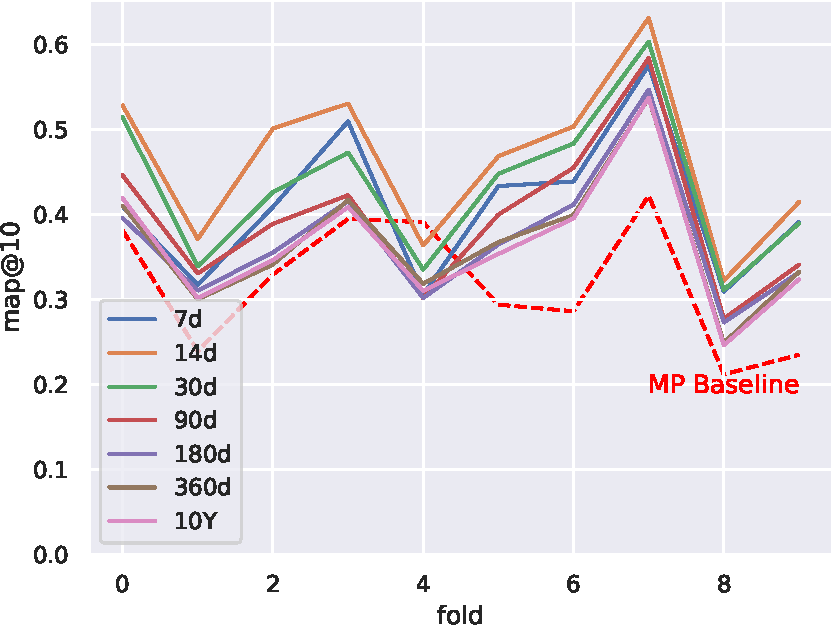
\includegraphics[width=\linewidth]{figures/04_implementacion/11_cosine_results_results-lines_W-THU_normalize=True.pdf}
        \caption{Precisión obtenida en cada fold.}
    \end{subfigure}\hfill\begin{subfigure}{.48\textwidth}
        \centering
        % Source: 11_pln-tune.ipynb [30]
        % Actualizado 2024-04-10
        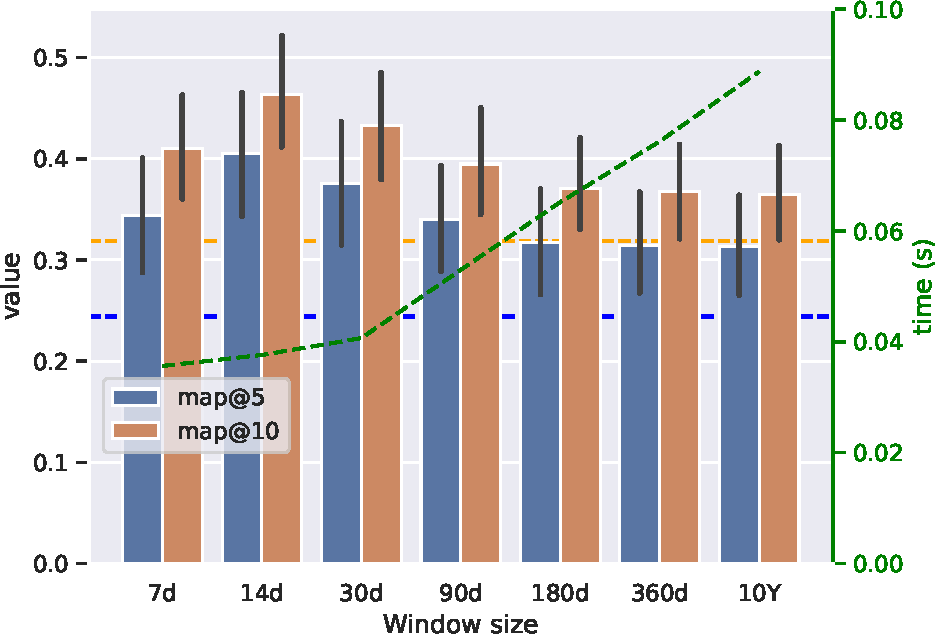
\includegraphics[width=\linewidth]{figures/04_implementacion/11_cosine_results_window-size_W-THU_normalize=True.pdf}
        \caption{Media entre todos los folds. Las barras de error representan el \acrshort{ic}.}
        \label{fig:pln-similarity_window-size}
    \end{subfigure}
    \caption[Resultados del sistema recomendador basado en similitud del coseno en Decentraland.]{Resultados del sistema recomendador basado en similitud con el usuario entre propuestas y usuarios dependiendo del tamaño de la ventana de propuestas en Decentraland. En rojo la línea base del clasificador más votado.}
    \label{fig:pln-similairity_results}
\end{figure}

% Source: 11_pln-tune.ipynb [26] Column 10 years
% Actualizado 2024-04-10
El rendimiento medio del MAP@10 de este recomendador en todos los folds es de $0.36\pm 0.08$. Se realizó un experimento para evaluar el impacto de reducir el número de propuestas utilizadas para realizar las recomendaciones y se observó que limitar las propuestas a aquellas en las que el usuario ha votado durante los últimos 30 días mejoraba significativamente la calidad de las recomendaciones en comparación con el uso de todo el conjunto de datos. Además, este enfoque reduce el tiempo de cálculo de los \textit{embeddings} del usuario debido a la menor cantidad de propuestas a considerar.

Se llevó a cabo una búsqueda en rejilla (\textit{grid search}) con diferentes tamaños de ventana, variando desde 7 días hasta 1 año. Los resultados se presentan en la figura~\ref{fig:pln-similairity_results}. Se observó que el uso de una ventana de 14 días resulta óptimo, ya que el $map@10$ aumenta de $0.36\pm 0.08$ a $0.46\pm 0.09$, en comparación con el uso de todo el conjunto de propuestas. Además, el tiempo de ejecución se reduce de 86ms a 36ms. Hay que tener en cuenta que el tiempo de ejecución no incluye el cálculo de los \textit{embeddings}, que está cacheado, aunque el servidor (véase~\ref{ch:servidor}) tarda a penas 5 segundos en calcular los \textit{embeddings} de las 1950 propuestas, utilizando el modelo \url{all-mpnet-base-v2}.

\subsubsection{K vecinos más cercanos}

% \begin{itemize}
%     \item Cada usuario tiene su propio modelo \gls{knn} en el que los datos son las propuestas en las que ha votado o no, y se intenta clasificar una propuesta nueva haciendo la agregación de los k vecinos más cercanos. Se ha utilizado la clase \url{KNeighborsClassifier} de scikit learn~\cite{pedregosa_scikit-learn_2011}.
%     \item Debido a que muchos usuarios han votado poco, se hace \textit{fallback} al modelo most popular en el caso de que el $k$ del \gls{knn} sea mayor que el número de propuestas en las que ha votado el usuario. Esto hace que cuanto mayor sea la $k$, se haga menos uso de \gls{knn} y más del fallback. 
%     \item Sin embargo, aumentar el tamaño de la ventana añade más propuestas al entrenamiento, por lo que aumenta el porcentaje de uso de knn. Ambos casos se ven ilustrados en la figura~\ref{fig:knn_usage}. Obviamente, cambiar la métrica utilizada no afectará al porcentaje de uso de \gls{knn}.
%     \item Además, debido a la baja cantidad de muestras negativas, habrá una sobre-representación de muestras. Por ello hacemos un sampling en el que el número de muestras negativas es igual al número de muestras positivas.
%     \item Hay que tener en cuenta que como el feedback es implícito, una muestra negativa no implica que al usuario no le hubiese interesado la propuesta, seguramente no haya votado en ella porque no estaba disponible en ese momento.
%     \item Es necesario hacer una búsqueda de hiperparámetros en k, además mantenemos lo del tamaño de la ventana. También se ha probado a usar tanto la distancia del coseno como la minkowski, realizando una búsqueda en una rejilla de 196 puntos, definida por el espacio de la tabla~\ref{tab:knn_espacio_busqueda}.
%     \item Sin embargo, da igual, pues a penas supera la línea base del más votado. Esto es debido a que tenemos muy poco feedback positivo, por lo que las muestras negativas en realidad son muy parecidas a otros vecinos positivos.
%     \item El resumen de los resultados de la búsqueda está en la figura~\ref{fig:knn_results_all}. En general, coger cualquiera de las dos maneras para medir la distancia no influye en los resultados, y el mejor valor de $k$ parece ser 1 independientemente del tamaño de la ventana. Cuando la $k$ es demasiado alta, acaba haciendo uso tan solo del fallback, que no realiza recomendaciones personalizadas. En cuanto al tamaño de la ventana, parece ser que lo mejor es coger las propuestas en las que el usuario ha votado en los últimos 360 días, contrastando con el de similitud con el usuario, en el que la mejor opción era coger tan sólo los últimos 14 días. La mejor opción (k=1, window=360d, metric=cosine) tiene como resultado un MAP@10 de $0.44\pm0.11$. Supera en 4 puntos al modelo de similitud con el usuario sin optimizar, pero la versión optimizada supera a este por 8 puntos.
%     \item Sobre el tiempo de ejecución (véase figura~\ref{fig:knn_results_time}), este modelo es 300 veces más lento que el modelo basado en similitud con el usuario, pasando del orden de los 50ms a 15 segundos. El otro modelo realiza una simple suma y calcula la distancia del usuario a todas las propuestas, mientras que este modelo necesita calcular la distancia de todas las propuestas entre sí. Y eso que he hecho sampling para quitar ejemplos negativos.
% \end{itemize}

En el enfoque de \acrfull{knn}, cada usuario posee su propio modelo donde los datos son las propuestas en las que ha votado o no. Se intenta clasificar una nueva propuesta en dos clases (votará/no votará) mediante la agregación de los $k$ vecinos más cercanos. El \textit{score} de una predicción será el porcentaje de vecinos de la nueva propuesta en los que el usuario ha votado. Para esto, se ha empleado la clase \url{KNeighborsClassifier} de scikit-learn~\cite{pedregosa_scikit-learn_2011}.

Dado el bajo número de muestras positivas, se realiza un muestreo donde el número de muestras negativas es igual al número de muestras positivas. Es importante destacar que, dado que el feedback es implícito, una muestra negativa no indica necesariamente que al usuario no le habría interesado la propuesta. Es probable que el usuario no haya votado en ella porque no estaba disponible en ese momento.

Debido a que muchos usuarios han emitido pocos votos, se realiza un \textit{fallback} al modelo línea base Más Popular (véase~\ref{sec:linea_base}) en el caso de que el valor de $k$ en el \gls{knn} sea mayor que el número de propuestas en las que ha votado el usuario. Esto implica que a medida que $k$ aumenta, se reduce el uso del \gls{knn} y se incrementa el del \textit{fallback}, como puede observarse en la figura~\ref{fig:knn_usage_k}.

\begin{figure}[t]
    \centering
    \begin{subfigure}{.48\textwidth}
        \centering
        % Source: 11_pln-tune.ipynb [42]
        % Actualizado 2024-04-10
        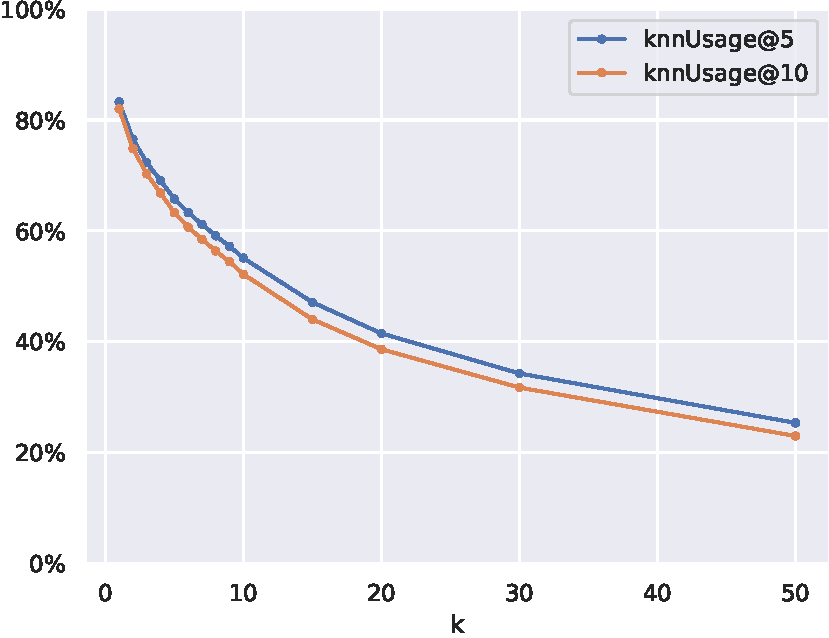
\includegraphics[width=\linewidth]{figures/04_implementacion/11_knn_usage_k_W-THU_normalize=True.pdf}
        \caption{Porcentaje medio de uso de knn para los distintos $k$ probados.}
        \label{fig:knn_usage_k}
    \end{subfigure}\hfill\begin{subfigure}{.48\textwidth}
        \centering
        % Source: 11_pln-tune.ipynb [43]
        % Actualizado 2024-04-10
        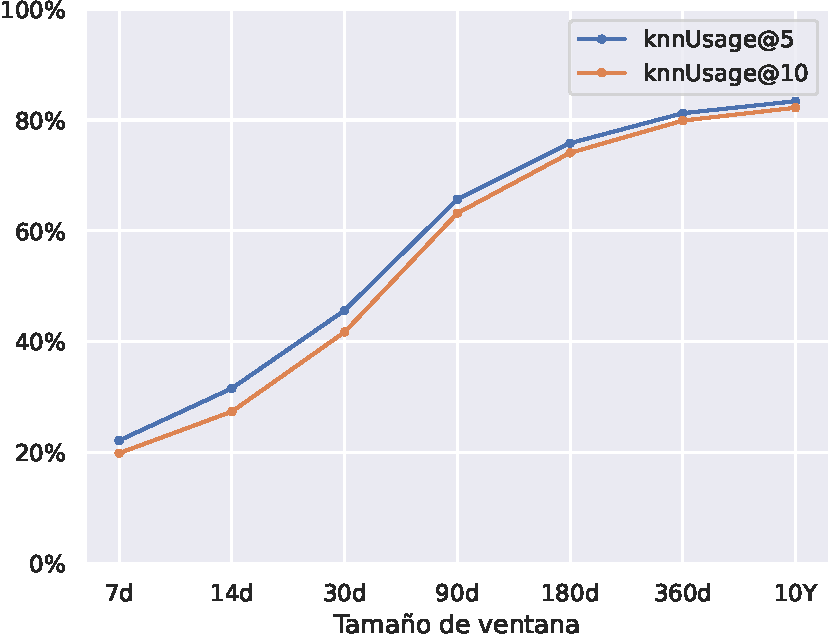
\includegraphics[width=\linewidth]{figures/04_implementacion/11_knn_usage_window_size_W-THU_normalize=True.pdf}
        \caption{Porcentaje medio de uso de knn en cada tamaño de ventana.}
        \label{fig:knn_usage_window_size}
    \end{subfigure}
    \caption[Porcentaje de uso de \acrshort{knn} vs el \textit{fallback} variando hiperparámetros.]{Porcentaje de uso de \gls{knn} vs el \textit{fallback} variando dos hiperparámetros.}
    \label{fig:knn_usage}
\end{figure}

Al igual que en el modelo anterior, se ha decidido probar distintas ventanas temporales de entrenamiento para comprobar el rendimiento del modelo. El tamaño de esta ventana impacta en la cantidad de propuestas incluidas en el entrenamiento, afectando así el porcentaje de uso del \gls{knn}. Este efecto se observa en la figura~\ref{fig:knn_usage_window_size}. También se ha probado el modelo con distintas métricas de distancia entre las muestras. Sin embargo, cambiar la métrica de distancia no afectará al porcentaje de uso del \gls{knn}.

Para utilizar \gls{knn}, es necesario llevar a cabo una búsqueda del hiperparámetro $k$. Además, usamos distintos tamaños de ventana de propuestas a considerar como en el modelo anterior, y probamos tanto con la distancia del coseno como la Euclídea (Minkowski con $p=2$). Se ha realizado la búsqueda con una rejilla de 196 puntos, definida por el espacio en la tabla~\ref{tab:knn_espacio_busqueda}.

\begin{table}
    \centering
    \begin{tabular}{l|c}
        \toprule
        \textbf{Hiperparámetro} & \textbf{Valores} \\
        \midrule
        Window size & $ \{ 7d,14d,30d,90d,180d,360d,10Y \} $ \\
        k vecinos & $ [1,10] \cup \{15,20,30,50\}$ \\
        Métrica & \{ Euclídea, Similitud del coseno \} \\
        \bottomrule
    \end{tabular}
    \caption{Espacio de búsqueda de hiperparámetros para la optimización del modelo basado en \gls{pln} y \gls{knn}.}
    \label{tab:knn_espacio_busqueda}
\end{table}

El resumen de los resultados de la búsqueda se muestra en la figura~\ref{fig:knn_results_all}. En general, la elección de la medida de distancia apenas influye en los resultados, y el mejor valor de $k$ parece ser 1 (\textit{Nearest neighbor}) independientemente del tamaño de la ventana. Además, cuando $k$ es demasiado alto, el modelo acaba recurriendo únicamente al \textit{fallback}, lo que no ofrece recomendaciones personalizadas.

En cuanto al tiempo de ejecución (véase figura~\ref{fig:knn_results_time}), este modelo es 300 veces más lento que el basado en similitud con el usuario, con tiempos de ejecución de alrededor de 15 segundos para los hiperparámetros que maximizan el \gls{map}. A diferencia del otro modelo, que realiza una simple suma y calcula la distancia del usuario a todas las propuestas, este necesita calcular la distancia entre todas las propuestas entre sí. Se ha realizado un muestreo para eliminar ejemplos negativos, lo que sugiere que el tiempo de ejecución podría ser aún mayor sin este proceso.

\begin{figure}
    \begin{minipage}{.48\textwidth}
        % Source: 11_pln-tune.ipynb [45]
        % Actualizado 2024-04-10
        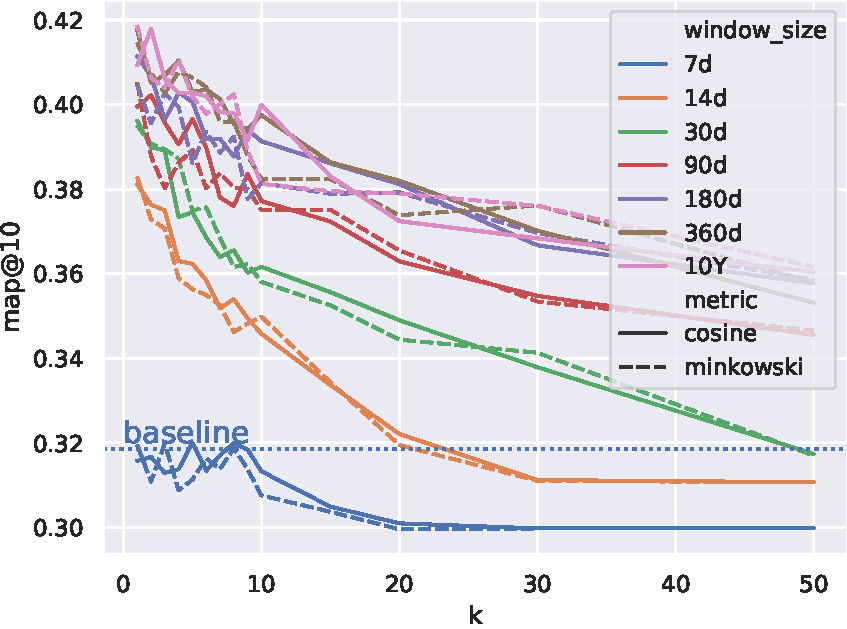
\includegraphics[width=\linewidth]{figures/04_implementacion/11_knn_results_all_W-THU_normalize=True.pdf}
        \caption{Resultados de la búsqueda de hiperparámetros para el modelo \acrshort{knn}}
        \label{fig:knn_results_all}
    \end{minipage}%
    \hfill%
    \begin{minipage}{.48\textwidth}
        % Source: 11_pln-tune.ipynb [46]
        % Actualizado 2024-04-10
        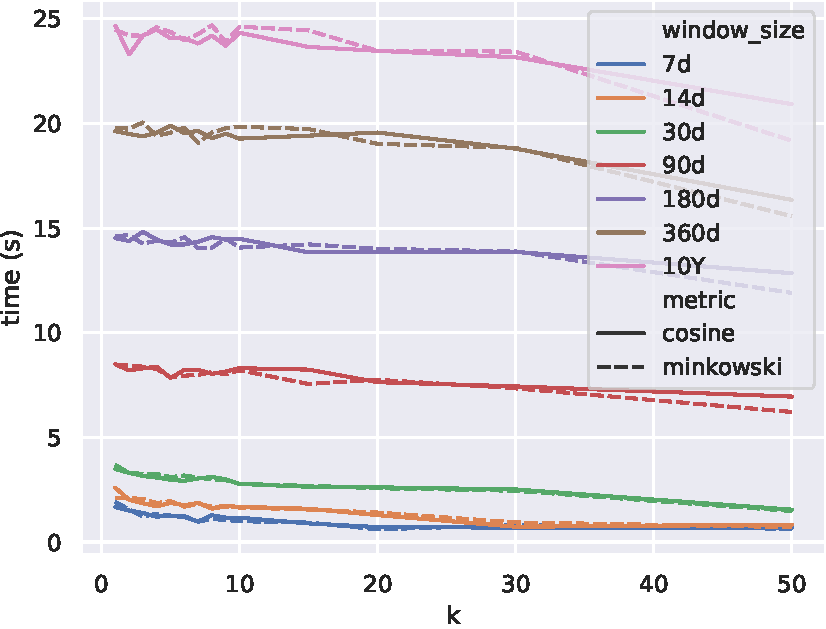
\includegraphics[width=\linewidth]{figures/04_implementacion/11_knn_results_time_W-THU_normalize=True.pdf}
        \caption{Tiempo de ejecución con varios hiperparámetros con el modelo \acrshort{knn}}
        \label{fig:knn_results_time}
    \end{minipage}
\end{figure}

\subsection{Sistema basado en filtrado colaborativo}
\label{subsec:implementacion-colaborativo}

Esta estrategia se basa en aprovechar el grafo de relaciones entre los usuarios como parte del \gls{sr}. Esta aproximación permite capturar conexiones sociales y patrones emergentes en la interacción entre usuarios, incluso cuando la información sobre las propuestas en sí es limitada. Sin embargo, estas propuestas se desenvuelven en comunidades, donde surgen dinámicas específicas y existen estructuras sociales latentes, al igual que en el caso del Software Libre~\cite{bird_latent_2008}.

En términos más específicos, se ha desarrollado un sistema de filtrado colaborativo basado en aprendizaje profundo, utilizando en particular una \acrfull{gnn}. La intención es poder expandir el grafo en el futuro incorporando otras interacciones de los usuarios, incluso aquellas que ocurren fuera de la organización o de otras \glspl{dapp}, como las transferencias de dinero. Para esta implementación, se ha optado por utilizar el modelo LightGCN~\cite{he_lightgcn_2020}, disponible en la librería microsoft/recommenders~\cite{argyriou_microsoft_2020}. Este modelo se ha seleccionado debido a su actualidad, rendimiento sólido, y su eficiencia computacional (similar a una factorización de matrices), además de haber sido probado en diversos conjuntos de datos y \textit{benchmarks}. 

Es importante subrayar que el propósito principal de este proyecto no radica en la creación ni en el desarrollo de nuevos modelos, sino en la aplicación de los \acrlongpl{sr} a las \glspl{dao}. El funcionamiento del modelo se explica en profundidad en la subsubsección~\ref{subsubsec:lightgcn}.

En cuanto al entrenamiento y ajuste de hiperparámetros del modelo, se ha utilizado la librería Ray Tune~\cite{liaw_tune_2018}. Ha sido necesario modificar ligeramente las siguientes partes de la implementación del modelo:

\begin{itemize}
    \item Se incorporó un post-filtrado que evita recomendar propuestas que no están abiertas. Para ello, se ajustó la función \texttt{recommend\_k\_items}, la cual ahora recibe una lista de propuestas \textit{recomendables} (es decir, actualmente abiertas). Aquellas recomendaciones que no estén en esta lista se les asigna un \textit{score} de $-\infty$, de ese modo al hacer el \textit{ranking} de propuestas aparecerán las últimas y no serán recomendadas.
    \item Se introdujo el método \texttt{fit\_epoch} para realizar el fit de una sola época, permitiendo la detención temprana y permitiendo reportar las métricas con mayor granularidad en Ray Tune.
\end{itemize}

Este modelo modificado está disponible en la clase \texttt{LightGCNCustom}, ubicada en el módulo \texttt{src.models.lightgcn} del repositorio del TFM en GitHub~\cite{davo_daviddavoupm-tfm-notebooks_2024}. 

El espacio de búsqueda de hiperparámetros es continuo, por lo que se realiza una búsqueda metaheurística en este espacio usando HyperOpt~\cite{bergstra_making_2013}, pues es el único algoritmo de búsqueda de Ray Tune que permite la búsqueda en un espacio que mezcle hiperparámetros con valores continuos y discretos. En la tabla~\ref{tab:lightgcn_espacio_busqueda} se muestran los valores que definen el espacio de búsqueda utilizado.

\begin{table}[tbh]
    \centering
    \begin{tabular}{l|cc}
        \toprule
        \textbf{Hiperparámetro} & \textbf{Valores} & \textbf{Muestreo} \\
        \midrule
        Batch size & $bs\in\{ 64, 128, 256, 512, 1024 \} $ & Uniforme \\
        Embedding dim & $e\in\mathbb{N}, 1 \leq e \leq 1024$ & Loguniforme \\
        Capas de convolución & $c\in \{1,2,3,4,5,6\} $ & Uniforme \\
        Learning rate & $lr\in\mathbb{R}, 10^{-4} \leq lr \leq 1$ & Loguniforme \\
        Regularización L2 & $l2\in\mathbb{R}, 10^{-7}\leq l2 \leq 10^{-2}$ & Loguniforme \\ 
        \bottomrule
    \end{tabular}
    \caption{Espacio de búsqueda de hiperparámetros para la optimización del modelo LightGCN.}
    \label{tab:lightgcn_espacio_busqueda}
\end{table}

Asumimos que el modelo se reentrena cada vez que se requiere actualizar las recomendaciones. En consecuencia, no tiene sentido utilizar el mismo conjunto de hiperparámetros para el modelo en diferentes folds; se considera posible ajustar los hiperparámetros para generar nuevas recomendaciones. Por lo tanto, se optimiza la búsqueda de hiperparámetros en cada uno de los folds.

Sobre la generación de estos folds, se proporciona una explicación detallada en la sección~\ref{sec:division_datos}. Para cada uno de los 10 folds, se realizan 100 muestras. Las primeras 20 muestras son el punto de partida de HyperOpt. Aunque normalmente se utilizan muestras aleatorias, uno de los puntos de inicio es la mejor muestra del fold anterior.

La búsqueda intenta maximizar la métrica objetivo MAP@10. Se observó que utilizar la función de pérdida \gls{bpr} generaba sobre-aprendizaje, ya que resultaba en un valor de pérdida muy bajo, pero la precisión no alcanzaba niveles aceptables por encima de la línea base. Además, intentar optimizar la precisión o exhaustividad tampoco daba buenos resultados al ignorar por completo el orden de las recomendaciones. Sin embargo, un mejor \gls{map} sí se corresponde con una mejor precisión, como puede verse en la figura~\ref{fig:scatter_map_precision}. También podría haberse usado el \gls{ndcg}, pues son métricas similares y que están correlacionadas, como puede observarse en la figura~\ref{fig:scatter_ndcg_map}.

\begin{figure}[bt]
    \begin{minipage}{.48\textwidth}
        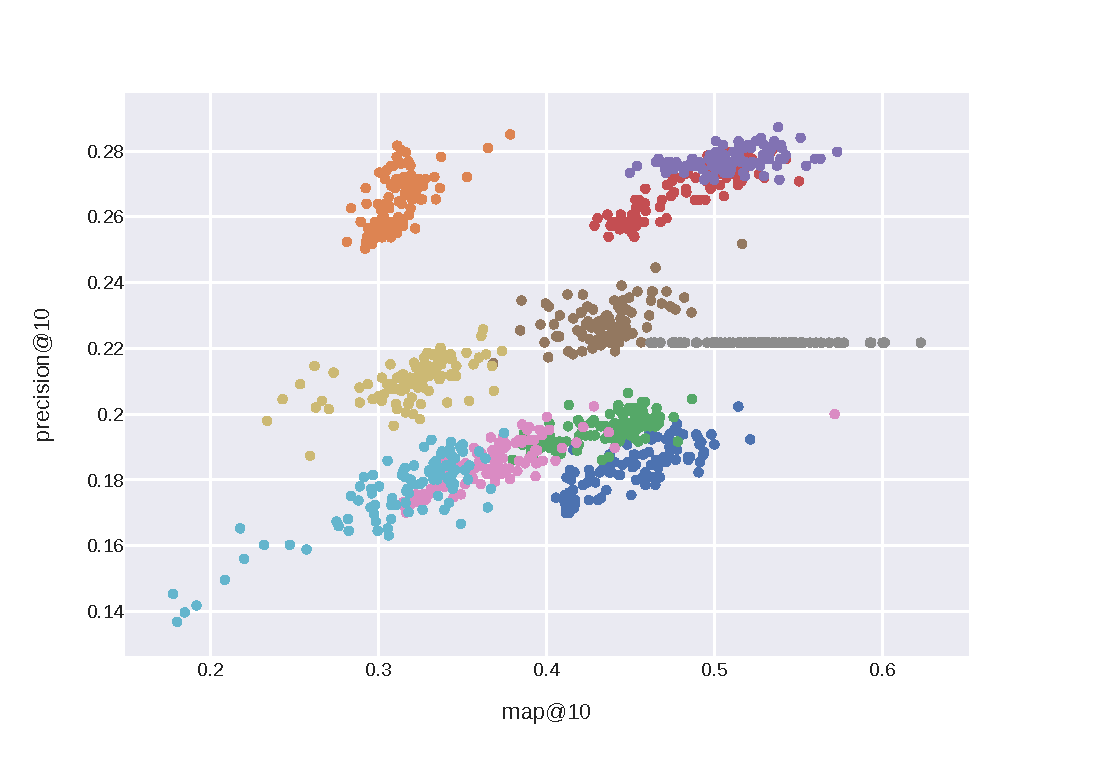
\includegraphics[width=\linewidth]{figures/04_implementacion/scatter_map_precision.pdf}
        \caption[Gráfico de dispersión entre el MAP y la precisión en las 1000 muestras tomadas del recomendador GNN para Decentraland.]{Gráfico de dispersión entre el \gls{map} y la precisión en las 1000 muestras tomadas para la optimización del recomendador basado en \gls{gnn} para la \gls{dao} Decentraland. Dentro de cada fold (color), aumentar el \gls{map} hace aumentar la precisión.}
        \label{fig:scatter_map_precision}
    \end{minipage}%
    \hfill%
    \begin{minipage}{.48\textwidth}
        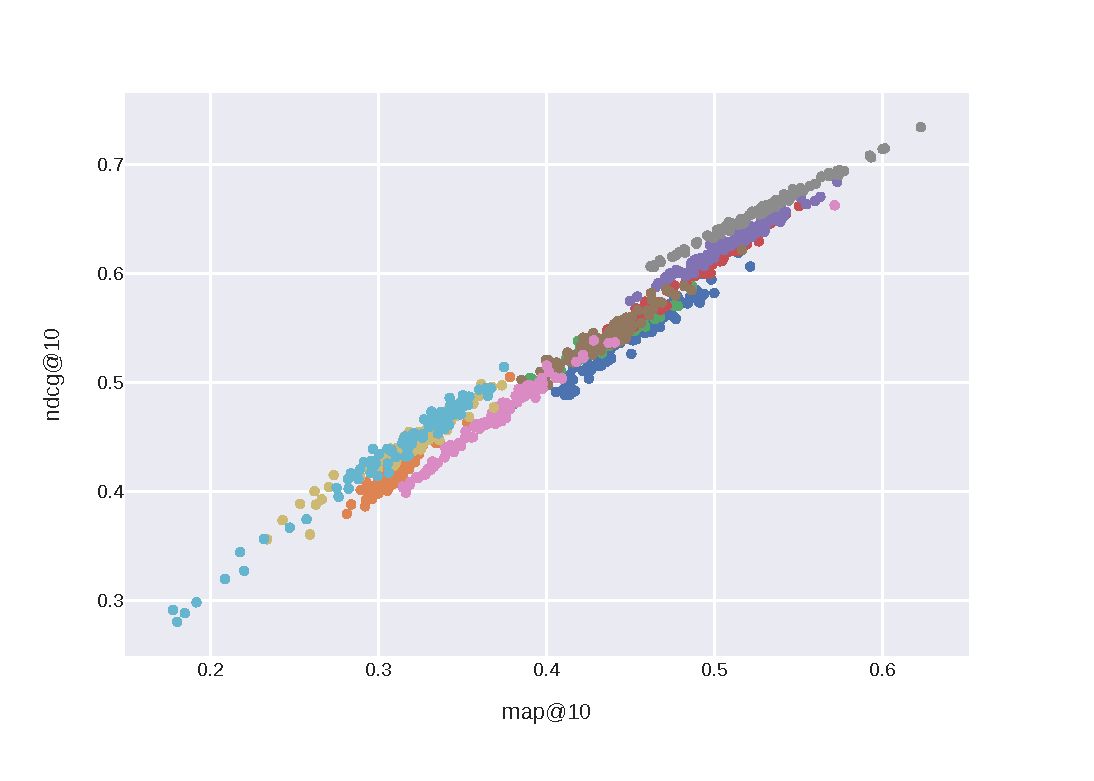
\includegraphics[width=\linewidth]{figures/04_implementacion/scatter_ndcg_map.pdf}
        \caption[Gráfico de dispersión entre el MAP y el nDCG en las 1000 muestras tomadas del recomendador GNN para Decentraland.]{Gráfico de dispersión entre el \gls{map} y el \gls{ndcg} en las 1000 muestras tomadas para la optimización del recomendador basado en \gls{gnn} para la \gls{dao} Decentraland. El color es distinto para cada uno de los folds, mostrando que cada fold tiene unas métricas máximas alcanzables distintas.}
        \label{fig:scatter_ndcg_map}
    \end{minipage}
\end{figure}

Todo el trabajo realizado se encuentra documentado en dos notebooks disponibles en el repositorio de GitHub del proyecto~\cite{davo_daviddavoupm-tfm-notebooks_2024}. El primero, denominado \url{07\_microsoft\_tuning.ipynb}, aborda la definición del proceso de entrenamiento del modelo. El segundo, \url{09\_analyze\_results}, presenta los resultados de la ejecución y genera las métricas y gráficas expuestas en las siguientes secciones.

La decisión de utilizar dos notebooks se tomó para permitir la ejecución en paralelo del segundo y monitorizar el estado de ejecución del primero, ya que el experimento en su totalidad requiere varias horas para completarse.

\subsubsection{Tiempo de ejecución}

El experimento se configura para realizar 100 muestras en 10 folds, con cada ejecución limitada a 5 minutos (300 segundos). Por ende, el tiempo de ejecución teórico asciende a 5,000 minutos, aproximadamente 3 días y medio. No obstante, en la práctica, la suma de los tiempos de ejecución de los experimentos es de 3 días y 20 horas. Esto se debe a que, en lugar de interrumpir abruptamente el experimento, se permite que no continúe tras concluir el \textit{epoch}, y el tiempo medio de ejecución se sitúa en 330 segundos.

El tiempo real de ejecución del experimento es de aproximadamente 5 horas y 45 minutos. Esto se debe a que el servidor utilizado (consultar el apéndice~\ref{ch:servidor}) permitía la ejecución de 16 entrenamientos en paralelo sin afectar el tiempo de ejecución de otros entrenamientos. 

\subsubsection{Emisiones del experimento}
Según la información proporcionada por el programa nvidia-smi, la tarjeta gráfica consumía 250W durante la ejecución de los experimentos. Además, de acuerdo con las especificaciones del procesador~\cite{intel_procesador_2022}, este tiene una potencia base de 150W, aunque no se estaba utilizando al 100\%.

Por lo tanto, la ejecución del experimento consumió 2.3KWh, equivalente a 0.23KWh por cada \textit{fold} como cota superior. En términos de emisiones, actualizar las recomendaciones resultaría en una emisión de 630g de $CO_2$ al utilizar una comercializadora en España sin \gls{gdo}~\cite{noauthor_anexo_2023}. En caso de actualizar las recomendaciones semanalmente, las emisiones ascenderían a aproximadamente 33kg de $CO_2$. Cabe destacar que, al ubicarse el servidor en la Facultad de Informática de la Universidad Complutense de Madrid, que ha adoptado electricidad de origen verde desde 2019, no se generan emisiones~\cite{vicerrectorado_de_tecnologia_y_sostenibilidad_informe_2021}.

\subsubsection{Evaluación del modelo}

No podemos emplear una búsqueda de hiperparámetros calculando el promedio de los resultados de todos los folds, ya que implicaría asumir dos supuestos cruciales: en primer lugar, que todos los modelos de cada fold deben tener los mismos hiperparámetros; y en segundo lugar, que los resultados de cada fold estarían disponibles para evaluar los anteriores.

Por lo tanto, optamos por realizar la optimización de hiperparámetros de manera independiente en cada fold. De las 100 muestras obtenidas durante la ejecución de la optimización de hiperparámetros de un fold, seleccionamos la mejor y la evaluamos utilizando dichos hiperparámetros en el siguiente fold.

Esta metodología busca simular el comportamiento de la optimización de hiperparámetros en un entorno real, donde se dispone de los datos hasta el momento actual pero se desconocen los datos futuros. Por ende, optimizamos los hiperparámetros utilizando únicamente los datos disponibles hasta el momento.

Es crucial resaltar que, para calcular la métrica objetivo de la optimización de hiperparámetros, utilizamos un conjunto de validación que, supuestamente, no está disponible en el momento del entrenamiento. Por esta razón, al modelo optimizado le llamamos \textquote{Oráculo}. Al modelo que emplea los hiperparámetros que obtienen la mejor métrica en el \textit{Oráculo} del fold anterior, lo denominamos \textquote{Realista}.

% https://en.wikibooks.org/wiki/LaTeX/Floats,_Figures_and_Captions
\begin{wrapfigure}{o}{.5\textwidth}
    \centering
    % Source: 09_analyze_results.ipynb [29]
    % Actualizado: 2024-04-10
    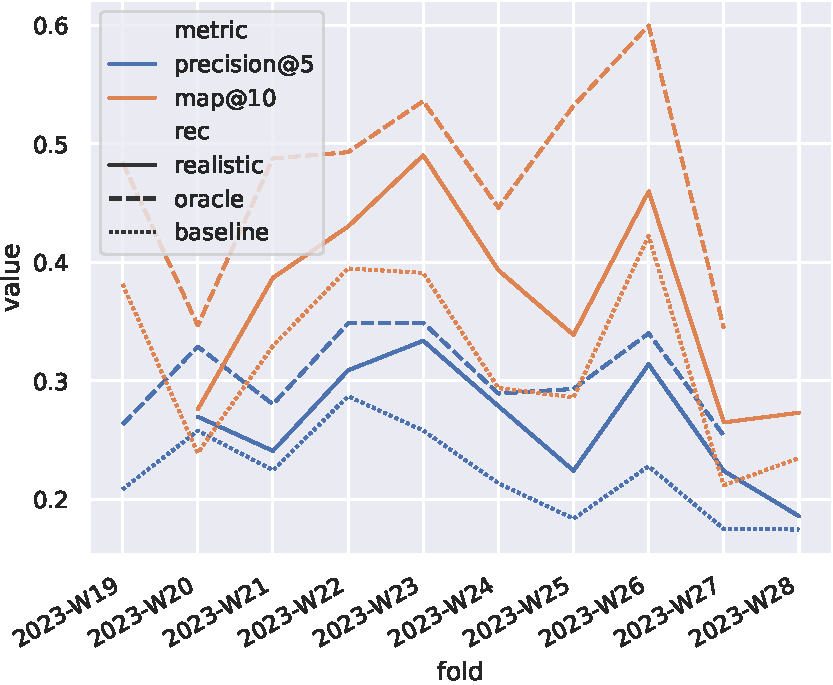
\includegraphics[width=\linewidth]{figures/04_implementacion/09_gnn_results.pdf}
    \caption[Resultados del entrenamiento realista del Sistema Recomendador basado en \textit{Graph Neural Networks}]{Resultados del entrenamiento \textit{realista} del \gls{sr} basado en \gls{gnn}.}
    \label{fig:gnn-realistic}
\end{wrapfigure}

% Source: 09_analyze_results.ipynb [29]
% Actualizado: 2024-04-10
En la figura~\ref{fig:gnn-realistic} se exponen los resultados de estas operaciones en los últimos 10 folds, comparando estos modelos con una línea base (recomendar las propuestas más votadas hasta el momento, véase~\ref{sec:linea_base}). La línea base arroja una MAP@10 media de $0.32\pm0.08$, mientras que el modelo Oráculo está altamente optimizado con un valor medio de $0.47\pm0.08$. El modelo Realista se posiciona entre ambos, con un valor de $0.37\pm0.08$. Aunque siempre es preferible utilizar el modelo Oráculo, el modelo Realista demuestra un rendimiento notable al superar en general a la línea base. En el capítulo~\ref{ch:resultados_discusion} se lleva a cabo una comparación entre los resultados obtenidos por el modelo Realista y el basado en \gls{pln} y el enfoque Híbrido.

\subsection{Sistema híbrido}
\label{subsec:implementacion-hybrid}

% \begin{itemize}
%     \item Es un sistema híbrido basado en la combinación de las recomendaciones de los dos sistemas presentados en los apartados anteriores.
%     \item Para la recomendación basada en contenido, se ha utilizado el modelo basado en la similitud del coseno con el embeding del usuario, en lugar del modelo \gls{knn}, debido a sus mejores resultados y rapidez.
%     \item Se han utilizado los hiperparámetros optimizados para los sistemas individuales, no se ha vuelto a realizar una búsqueda de hiperparámetros en el híbrido.
%     \item Para combinar los resultados, se piden $k$ recomendaciones a cada uno de los sistemas, y se entremezclan para formar un conjunto de $k$ recomendaciones. En caso de haber recomendaciones duplicadas, en las que coinciden ambos sistemas, podemos distinguir tres métodos de fusión, que se detallarán en la siguiente sección.
% \end{itemize}

El sistema híbrido propuesto combina las recomendaciones generadas por los dos sistemas presentados en los apartados anteriores. En lugar del modelo \gls{knn} utilizado en la recomendación basada en contenido, se optó por emplear el modelo basado en la similitud del coseno con el \textit{embedding} del usuario, debido a su mejor desempeño y rapidez. Se emplearon los hiperparámetros optimizados para cada sistema individual, Sin realizar una búsqueda adicional de hiperparámetros para el sistema híbrido. El código de este modelo se encuentra en la clase \url{src.models.hybrid.HybridRecommendation}, y se ha evaluado su funcionamiento en el notebook \url{12_hybrid.ipynb}.

Para combinar los resultados de ambos sistemas, se solicitan $k$ recomendaciones a cada uno y se intercalan para formar un conjunto de $k$ recomendaciones. En caso de que existan recomendaciones duplicadas, es decir, aquellas en las que coinciden ambos sistemas, se han definido tres métodos de fusión, que se detallarán en la siguiente subsección. En la figura~\ref{fig:metodos-fusion} ofrece una visualización de estos tres métodos.

\subsubsection{Métodos de fusión}

\begin{figure}[bth]
    \centering
    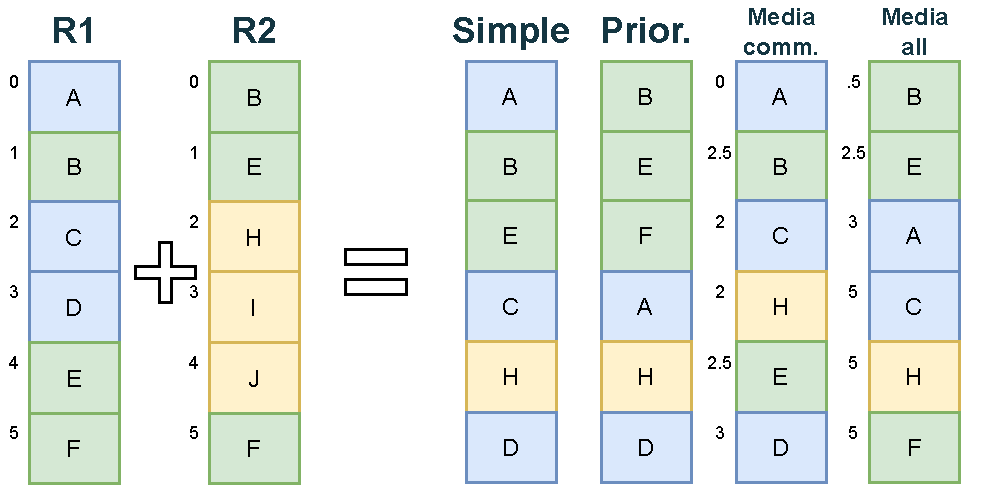
\includegraphics[width=\linewidth]{figures/04_implementacion/metodos-fusion.drawio.pdf}
    \caption[Visualización de los distintos métodos de fusión implementados de dos grupos de recomendaciones.]{Visualización de los distintos métodos de fusión implementados de dos grupos de recomendaciones. En azul las recomendaciones exclusivas al primer recomendador, en amarillo las recomendaciones exclusivas del segundo, y en verde las recomendaciones comunes. Una recomendación superior será una recomendación igual o mejor que la inferior, aunque no son comparables entre recomendadores. El número de la izquierda indica la posición, o el \textit{score} del sistema basado en la posición media.}
    \label{fig:metodos-fusion}
\end{figure}

% \begin{itemize}
%     \item La fusión de los dos sistemas recomendadores está basada en el entrelazamiento de las recomendaciones de ambos. Es decir, se coje una recomendación de cada uno hasta llegar a $k$.
%     \item Sin embargo, según como tratemos a las recomendaciones que aparecen en ambos, podemos distinguir tres métodos, que puede visualizarse su funcionamiento en la figura~\ref{fig:metodos-fusion}.
% \end{itemize}

La fusión de los dos sistemas recomendadores se basa en el entrelazamiento de las recomendaciones de ambos, es decir, se selecciona una recomendación de cada sistema hasta alcanzar $k$. Sin embargo, la manera en que tratamos las recomendaciones que aparecen en ambos sistemas puede variar, y a continuación se describen cuatro métodos de tratar estos duplicados:


\paragraph*{Entrelazado simple}

Se realiza el entrelazado de las recomendaciones y luego se eliminan los elementos duplicados. Es decir, la prioridad asignada a un elemento común será la máxima de las prioridades generadas por los dos recomendadores.

\paragraph*{Priorizar los comunes}

Se priorizan primero los elementos comunes, asumiendo que si ambos recomendadores coinciden en una recomendación, es porque se considera una buena opción. Los elementos no comunes, son entrelazados.

\paragraph*{Posición media de los comunes}

Se calcula la posición media de los elementos comunes en ambos sistemas, y luego se seleccionan los elementos según su \textit{ranking} en esta posición media. Los elementos que no son comunes no varían su \textit{puntuación}. Un elemento duplicado que aparece en la primera posición de un recomendador y en la tercera del otro, tendrá una puntuación de 1, por lo que debería aparecer entre el primero y el segundo.

\paragraph*{Posición media}

% \begin{itemize}
%     \item Las recomendaciones que aparezcan en un solo recomendador seguramente no sean tan buenas. 
%     \item Por lo tanto, también se hace la media de sus posiciones, pero como no conocemos la posición en la que está en el otro recomendador, asumimos que estaría en la posición $i+k$ del otro recomendador.
%     \item Es decir, la posición de los comunes es la media, y la de los no comunes es penalizada sumandole $k/2$
% \end{itemize}

Al igual que en el método anterior, se calcula la posición media de los elementos comunes entre ambos sistemas. Sin embargo, como asumimos que las recomendaciones que no aparecen en ambos sistemas puede que no sean tan buenas, también se calcula su posición media. Como no se conoce la posición real en el otro recomendador, se asume que estarían en la posición $i+k$, donde $i$ es la posición en el recomendador en el que aparecen, y $k$ es el número de elementos comunes. Es decir, se penaliza la posición de los elementos no comunes agregándoles $k/2$ a su posición.

\subsubsection{Evaluación del recomendador híbrido}

% \begin{itemize}
%     \item El sistema híbrido combina los resultados de ambos así que, seguramente, más que mejorar, conseguirá una métrica intermedia, pero probablemente más estable.
%     \item Conforme se va aumentando la $k$ del número de recomendaciones, aparecen más recomendaciones repetidas y, por lo tanto, el método de fusión será cada vez menos relevante. Sin embargo, de realizar 5 recomendaciones, el 50\% serán exclusivas de cada recomendador, como puede verse en la figura~\ref{fig:hybrid-common-proposals}.
%     \item Como puede verse en la figura~\ref{fig:hybrid-fusion-results}, el método de fusión que más beneficia a los comunes es, obviamente, el que prioriza a los comunes. Además, todos los métodos benefician ligeramente (hasta en $1/k$) al recomendador basado en \gls{pln}, pues cuando se hace el entremezclado, siempre se empieza por este y puede haber uno más.
%     \item Por cierto, el método que hace la media solo con los comunes y el del entrelazado puro (\textit{naive}) parece que tienden a escoger poco las recomendaciones comunes.
%     \item Además, con 10 recomendaciones se suelen coger tantas recomendaciones comunes que el método de fusión a penas afecta en que recomendador se elige.
%     \item Debido a que el recomendador basado en contenido es ligeramente mejor que el otro, el mejor método será el que priorice a este, aunque debido a la gran cantidad de recomendaciones comunes, saldrán resultados similares.
%     \item En la tabla \ref{tab:hybrid-fusion-results} podemos ver los resultados de los cuatro métodos, donde se observa que el mejor es el \textit{naive} por poco, ya que es el que más utiliza los resultados del nlp. Parece ser que, de hecho, podría ser mejor utilizar los resultados del nlp no-comunes y penalizar los comunes, ya que el recomendador basado en \gls{gnn} es peor.
%     \item En la figura~\ref{fig:hybrid-fusion-results-folds} se muestran los resultados de cada uno de los métodos fold a fold. El mejor método varía mucho dependiendo de como sean los datos de entrada, pero aun así excepto \textit{prioritize}, que parece más alocado, todos van de la mano y son similares.
% \end{itemize}

El enfoque híbrido propuesto combina los resultados de los \glspl{sr} basados en contenido y en filtrado colaborativo, buscando alcanzar un equilibrio entre ambos enfoques. Este método podría proporcionar un resultado intermedio entre los resultados individuales de cada sistema, aumentando la estabilidad de las recomendaciones.

Al incrementar el número de recomendaciones generadas ($k$), es probable que aumente la cantidad de recomendaciones duplicadas entre los sistemas. A medida que se generan más recomendaciones, disminuye la relevancia del método elegido para fusionar los dos sistemas. Con tan sólo 5 recomendaciones, el 50\% son comunes entre ambos sistemas, y con 10 este número aumenta al 74\%, como se puede observar en la figura~\ref{fig:hybrid-common-proposals}. De hecho, la precisión solo varía en una centésima según el método elegido (tabla~\ref{tab:hybrid-fusion-results}). Sin embargo, sí que será relevante la manera en la que se ordenan estas recomendaciones comunes para el \gls{map} y el \gls{ndcg}.

% LAS DOS FIGURAS LADO A LADO
% \begin{figure}
%     \begin{minipage}{.48\textwidth}
%         \centering
%         \includegraphics[width=\linewidth]{figures/04_implementacion/12_hybrid_common__Decentraland_W-THU_normalize=True.pdf}
%         \caption{Porcentaje de propuestas en común entre el recomendador basado en contenido y el de filtrado colaborativo aumentando el número de recomendaciones.}
%         \label{fig:hybrid-common-proposals}
%     \end{minipage}%
%     \hfill%
%     \begin{minipage}{.48\textwidth}
%         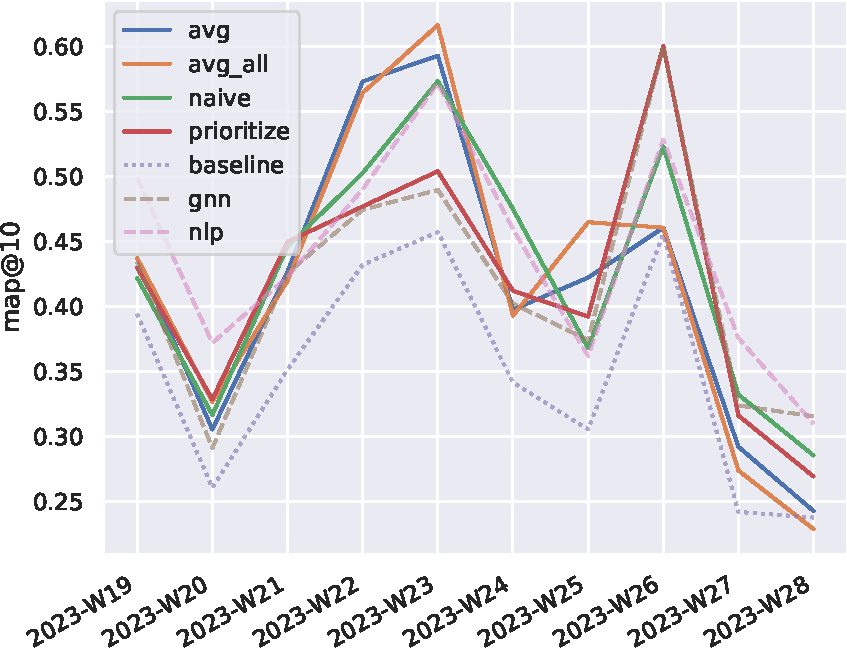
\includegraphics[width=\linewidth]{figures/04_implementacion/12_hybrid_merge_results_folds_Decentraland_W-THU_normalize=True.pdf}
%         \caption{Resultados del sistema recomendador híbrido que usa los distintos métodos de fusión en cada fold.}
%         \label{fig:hybrid-fusion-results-folds}
%     \end{minipage}
% \end{figure}

% SIDE CAPTION
\begin{SCfigure}
    \centering
    \caption[Porcentaje de propuestas en común entre los dos recomendadores base.]{Porcentaje de propuestas en común entre el recomendador basado en contenido y el de filtrado colaborativo aumentando el número de recomendaciones.}
    % Source: 12_hybrid.ipynb [20]
    % Actualizado: 2024-04-10
    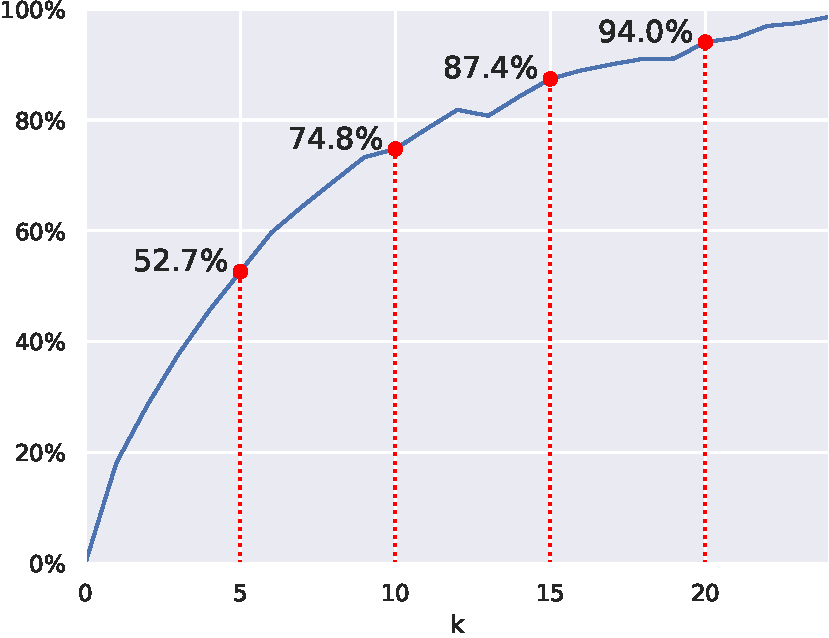
\includegraphics[width=.4\linewidth]{figures/04_implementacion/12_hybrid_common_Decentraland_W-THU_normalize=True.pdf}
    \label{fig:hybrid-common-proposals}
\end{SCfigure}
\begin{table}
    \centering
    \small
    % 12_hybrid.ipynb [25]
    % Actualizado: 2024-04-10
    \begin{tabular}{@{} l *{8}{S[table-format=1.3]} @{}}
        \toprule
          & 
         \multicolumn{2}{c}{precision@k} & 
         \multicolumn{2}{c}{recall@k} &
         \multicolumn{2}{c}{MAP@k} &
         \multicolumn{2}{c}{nDCG@k}
         \\
        % \cmidrule(r{5pt}){2-3}\cmidrule(l{5pt}){4-5}
        \textbf{Model} & 
        \multicolumn{1}{c}{k=5} & 
        \multicolumn{1}{c}{k=10} & 
        \multicolumn{1}{c}{k=5} & 
        \multicolumn{1}{c}{k=10} & 
        \multicolumn{1}{c}{k=5} & 
        \multicolumn{1}{c}{k=10} & 
        \multicolumn{1}{c}{k=5} & 
        \multicolumn{1}{c}{k=10}
        \\
        \midrule
         % avg & 0.416 & 0.113 & 0.360 & 0.095 \\
         % avg\_all & 0.417 & 0.122 & 0.357 & 0.087 \\
         % naive & \textbf{0.435} & \textbf{0.097} & \textbf{0.365} & \textbf{0.087} \\
         % prioritize & 0.431 & 0.106 & 0.357 & 0.093 \\ \hline
         % baseline & 0.348 & 0.085 & 0.274 & 0.074 \\
         % gnn & 0.425 & 0.010 & 0.352 & 0.097 \\
         % nlp & 0.439 & 0.084 & 0.364 & 0.083 \\

         % PRE 2024-04-10
        %  avg & 0.416 & 0.113 & 0.360 & 0.095 & 0.229 & 0.041 & 0.296 & 0.058 \\
        % avg\_all & 0.417 & 0.122 & 0.357 & 0.087 & 0.227 & 0.042 & 0.297 & 0.056 \\
        % naive & \textbf{0.435} & 0.097 & \textbf{0.365} & 0.087 & 0.228 & 0.042 & 0.298 & 0.057 \\
        % prioritize & 0.431 & 0.106 & 0.357 & 0.093 & 0.228 & 0.041 & 0.299 & 0.058 \\ \hline
        % baseline & 0.348 & 0.085 & 0.274 & 0.074 & 0.203 & 0.036 & 0.242 & 0.047 \\
        % gnn & 0.425 & 0.100 & 0.352 & 0.097 & 0.223 & 0.040 & 0.288 & 0.055 \\
        % pln & 0.439 & 0.084 & 0.364 & 0.083 & 0.229 & 0.040 & 0.299 & 0.066 \\
 OpenPop    & 0.221 & 0.196 & 0.351 & 0.626 & 0.236 & 0.310 & 0.317 & 0.416 \\
 \hline
 avg. all   & 0.292 & 0.222 & 0.526 & 0.751 & 0.347 & 0.398 & 0.458 & 0.515 \\
 avg.       & 0.287 & 0.224 & 0.514 & 0.759 & 0.341 & 0.399 & 0.449 & 0.518 \\
 prioritize & 0.291 & 0.224 & 0.525 & 0.755 & 0.341 & 0.399 & 0.452 & 0.520 \\
 naive      & 0.289 & 0.224 & 0.521 & 0.757 & 0.353 & 0.426 & 0.460 & 0.540 \\
 \hline
 GNN        & 0.271 & 0.216 & 0.485 & 0.736 & 0.334 & 0.409 & 0.434 & 0.522 \\
 NLP        & 0.295 & 0.227 & 0.513 & 0.765 & 0.357 & 0.434 & 0.464 & 0.549 \\
    \bottomrule
    \end{tabular}
    \caption{Resultados media de los distintos métodos de fusión del sistema recomendador híbrido y comparación con línea base y los otros dos sistemas recomendadores.}
    \label{tab:hybrid-fusion-results}
\end{table}

Todos los métodos benefician ligeramente al sistema basado en \gls{pln}, debido a que es seleccionado primero durante el entrelazado en el proceso de fusión, como puede verse en la figura~\ref{fig:hybrid-fusion-results}. Debido a que este es el mejor sistema de los dos, el método que más priorice las propuestas del \gls{pln} sobre las otras dará mejores resultados. El método que más elige las propuesas comunes es, obviamente, \textit{prioritize}, seguido de avg\_all, los dos métodos pesimistas sobre las recomendaciones realizadas por uno solo de los sistemas. Parece que el mejor de todos es \textit{naive}, que podríamos considerar que en lugar de agregar utilizando la operación \textit{media} utiliza la operación \textit{máximo}. Puede que este sea el mejor método (tabla~\ref{tab:hybrid-fusion-results}) porque tiende un poco más a escoger propuestas del recomendador \gls{pln}. Como puede verse en la figura, al aumentar el número de recomendaciones de 5 a 10, el método de fusión es menos relevante, pues siempre hay más de un 65\% de recomendaciones en común.

Finalmente, como se puede observar en la tabla~\ref{tab:hybrid-fusion-results} el recomendador híbrido tiene unos resultados entre medias de los dos recomendadores que lo forman, aunque en el map@5 supera al pln por una centésima.

Sin embargo, como se puede ver en la figura~\ref{fig:hybrid-fusion-results-folds} en el fold W19 el método \textit{proritize} supera al naive en map@10, y en los folds W22 y W23 es el \textit{avg} el que lo supera. Por lo tanto, el sistema recomendador híbrido podría superar a ambos de elegir de mejor manera cual de los dos sistemas base priorizar. La figura~\ref{fig:hybrid-best-results-folds} muestra los resultados de el mejor de los híbridos y los compara con los otros sistemas. El sistema \textit{naive}, que obtiene los mejores resultados de media, se encuentra entre los resultados del modelo GNN y el NLP excepto en el fold W23. En esta figura también se muestra con un sombreado azul los mejores y peores resultados obtenido por cualquier método de fusión, y en este caso sí que se supera en varios folds al modelo NLP. De hecho, de escoger en cada caso el mejor método de fusión, se conseguiría un MAP@10 medio de 0.437, superando en 3 centésimas al modelo NLP y demostrando que una mejor hibridación podría llegar a superar los resultados de ambos modelos base desarrollados.

\begin{figure}
    \centering
    % Source: 12_hybrid.ipynb [30]
    % Actualizado: 2024-04-10
    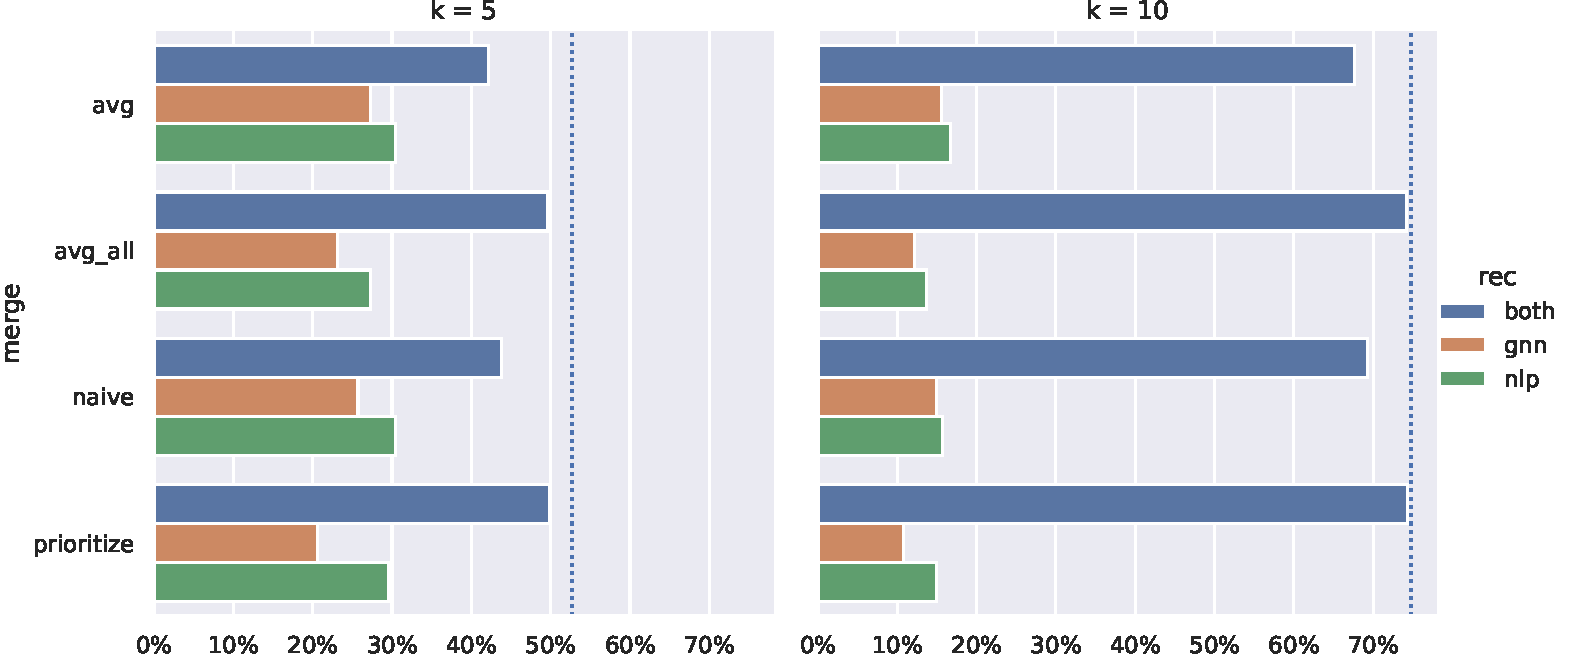
\includegraphics[width=\linewidth]{figures/04_implementacion/12_hybrid_merge_usage_Decentraland_W-THU_normalize=True.pdf}
    \caption[Porcentaje de propuestas de cada recomendador elegidas por cada uno de los métodos de fusión del recomendador híbrido.]{Porcentaje de propuestas de cada recomendador elegidas por cada uno de los métodos de fusión del recomendador híbrido (media de todos los folds). En las 5 recomendaciones originales, el porcentaje de propuestas duplicadas es 50.6\%, y con 10 recomendaciones hay un 74\% de propuestas duplicadas.}
    \label{fig:hybrid-fusion-results}
\end{figure}

\begin{figure}[p]
    \centering
    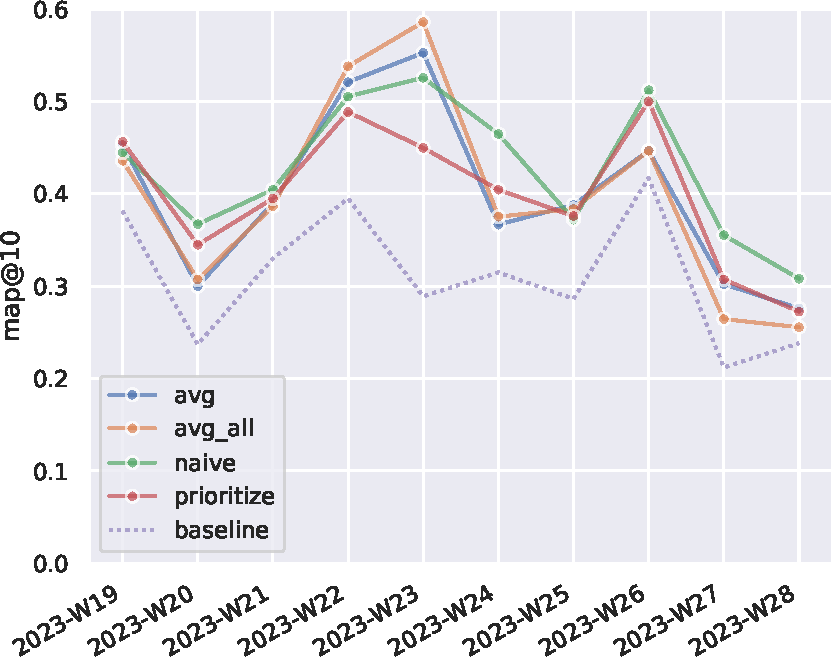
\includegraphics[width=.7\linewidth]{figures/04_implementacion/12_hybrid_merge_results_folds_Decentraland_W-THU_normalize=True_simple.pdf}
    \caption[Resultados del sistema recomendador híbrido que usa los distintos métodos de fusión en cada fold]{Resultados del sistema recomendador híbrido que usa los distintos métodos de fusión en cada fold, comparado con la línea base OpenPop.}
    \label{fig:hybrid-fusion-results-folds}
\end{figure}
\begin{figure}[p]
    \centering
    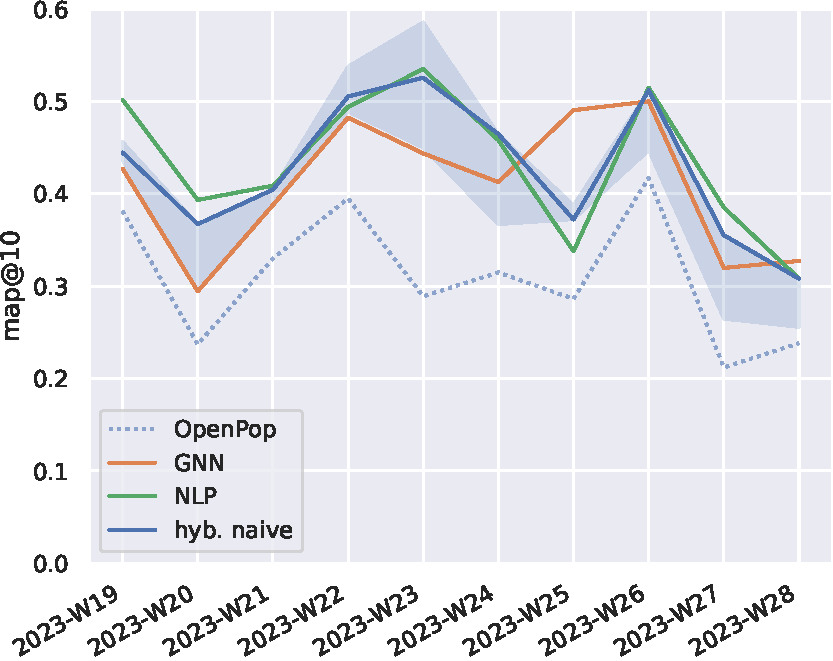
\includegraphics[width=.7\linewidth]{figures/04_implementacion/12_hybrid_merge_results_folds_Decentraland_W-THU_normalize=True_compare.pdf}
    \caption[Comparación del mejor híbrido con otros sistemas recomendadores.]{Resultados del sistema recomendador híbrido \textit{naïve} comparado con los otros sistemas recomendadores desarrollados. El área azul representa el mejor y peor resultado obtenido en ese fold por cualquiera de los otros métodos de fusión.}
    \label{fig:hybrid-best-results-folds}
\end{figure}
